\documentclass[a4paper,12pt,twoside,openany]{report}
%
% Wzorzec pracy dyplomowej
% J. Starzynski (jstar@iem.pw.edu.pl) na podstawie pracy dyplomowej
% mgr. inż. Błażeja Wincenciaka
% Wersja 0.1 - 8 października 2016
%
\usepackage{helvet}
\usepackage[T1]{fontenc}
\usepackage{anyfontsize}
\usepackage[utf8]{inputenc}
\usepackage[pdftex]{graphicx}
\usepackage{tabularx}
\usepackage{array}
\usepackage[english]{babel}
\usepackage{subfigure}
\usepackage{amsfonts}
\usepackage{verbatim}
\usepackage{indentfirst}
\usepackage[pdftex]{hyperref}


% rozmaite polecenia pomocnicze
% gdzie rysunki?
\newcommand{\ImgPath}{.}

% oznaczenie rzeczy do zrobienia/poprawienia
\newcommand{\TODO}{\textbf{TODO}}


% wyroznienie slow kluczowych
\newcommand{\tech}{\texttt}

% na oprawe (1.0cm - 0.7cm)*2 = 0.6cm
% na oprawe (1.1cm - 0.7cm)*2 = 0.8cm
%  oddsidemargin lewy margines na nieparzystych stronach
% evensidemargin lewy margines na parzystych stronach
\def\oprawa{1.05cm}
\addtolength{\oddsidemargin}{\oprawa}
\addtolength{\evensidemargin}{-\oprawa}

% table span multirows
\usepackage{multirow}
\usepackage{enumitem}	% enumitem.pdf
\setlist{listparindent=\parindent, parsep=\parskip} % potrzebuje enumitem

%%%%%%%%%%%%%%% Dodatkowe Pakiety %%%%%%%%%%%%%%%%%
\usepackage{prmag2017}   % definiuje komendy opieku,nrindeksu, rodzaj pracy, ...


%%%%%%%%%%%%%%% Strona Tytułowa %%%%%%%%%%%%%%%%%
% To trzeba wypelnic swoimi danymi
\title{Zdecentralizowana aplikacja do pożyczek na platformie Ethereum}

% autor
\author{Adam Kasperowicz}
\nrindeksu{279046}

\opiekun{dr hab. inż. Bartosz Sawicki}
\terminwykonania{1 lutego 2017} % data na oświadczeniu o samodzielności
\rok{2018}

% To sa domyslne wartosci
% - mozna je zmienic, jesli praca jest pisana gdzie indziej niz w ZETiIS
% - mozna je wyrzucic jesli praca jest pisana w ZETiIS
%\miasto{Warszawa}
%\uczelnia{POLITECHNIKA WARSZAWSKA}
%\wydzial{WYDZIAŁ ELEKTRYCZNY}
%\instytut{INSTYTUT ELEKTROTECHNIKI TEORETYCZNEJ\linebreak[1] I~SYSTEMÓW INFORMACYJNO-POMIAROWYCH}
% \zaklad{ZAKŁAD ELEKTROTECHNIKI TEORETYCZNEJ\linebreak[1] I~INFORMATYKI STOSOWANEJ}
%\kierunekstudiow{INFORMATYKA}

% domyslnie praca jest inzynierska, ale po odkomentowaniu ponizszej linii zrobi sie magisterska
%\pracamagisterska
%%% koniec od P.W

%\opinie{%
%  \newpage
\begin{center}
 {\large\bf  Opinia} \\
o pracy dyplomowej magisterskiej wykonanej przez dyplomanta\\
{\bf Zdolnego Studenta i Pracowitego Kolegę} \\
 Wydział Elektryczny, kierunek Informatyka,  Politechnika Warszawska\\
Temat pracy\\
\textit{\bf
TYTUŁ PRACY DYPLOMOWEJ
}\\
\end{center}
\medskip
\noindent
Promotor: {\bf dr inż. Miły Opiekun}\\
Ocena pracy dyplomowej: {\bf bardzo dobry}

\medskip

\centerline{\bf Treść opinii}
   Celem pracy dyplomowej panów dolnego Studenta i Pracowitego Kolegi  było
opracowanie systemu pozwalającego symulować  i opartego o oprogramowanie o
otwartych źródłach (ang. Open Source). Jak piszą Dyplomanci, starali się opracować
system, który łatwo będzie dostosować do zmieniających się dynamicznie wymagań,
będzie miał niewielkie wymagania sprzętowe i umożliwiał dalszą łatwą rozbudowę oraz
dostosowanie go do potrzeb.
Przedstawiona do recenzji praca składa się z krótkiego wstępu jasno i
wyczerpująco opisującego oraz uzasadniającego cel pracy, trzech rozdziałów (2-4)
zawierających opis istniejących podobnych
rozwiązań, komponentów rozpatrywanychjako kandydaci do
tworzonego systemu i wreszcie zagadnień wydajności wirtualnych
rozwiązań. Piąty rozdział to opis przygotowanego przez
Dyplomantów środowiska obejmujący opis konfiguracji
środowiska oraz przykładowe ćwiczenia laboratoryjne. Ostatni
rozdział pracy to opis możliwości dalszego
rozwoju projektu. W ramach przygotowania pracy Dyplomanci zebrali i przedstawili w
bardzo przejrzysty sposób duży zasób informacji, co świadczy o dobrej orientacji
w nowoczesnej i ciągle intensywnie rozwijanej tematyce stanowiącej
zakres pracy i o umiejętności przejrzystego przedstawienia tych
wyników. Praca zawiera dwa dodatki, z których pierwszy obejmuje wyniki
eksperymentów i badań nad wydajnością, a drugi to źródła
skryptów budujących środowisko.

 Dyplomanci dość
dobrze zrealizowali postawione przed nimi zadanie,
wykazali się więc umiejętnością zastosowania w praktyce wiedzy
przedstawionej w rozdziałach 2-4.  Uważam, że cele postawione w założeniach pracy zostały pomyślnie
zrealizowane. Proponuję ocenę bardzo dobrą (5).

\vskip 1cm
{
\raggedleft
(data, podpis)\kern1cm

}
%  \newpage
%  \newpage
\begin{center}
 {\large\bf  Recenzja } \\
pracy dyplomowej magisterskiej wykonanej przez dyplomanta\\
{\bf Zdolnego Studenta i Pracowitego Kolegę} \\
 Wydział Elektryczny, kierunek Informatyka,  Politechnika Warszawska\\
Temat pracy\\
\textit{\bf
TYTUŁ PRACY DYPLOMOWEJ
}\\
\end{center}
\medskip
\noindent
Recenzent: {\bf prof. nzw. dr hab. inż. Jan Surowy}\\
Ocena pracy dyplomowej: {\bf bardzo dobry}
\medskip


\centerline{\bf Treść recenzji}
   Celem pracy dyplomowej panów dolnego Studenta i Pracowitego Kolegi  było
opracowanie systemu pozwalającego symulować  i opartego o oprogramowanie o
otwartych źródłach (ang. Open Source). Jak piszą Dyplomanci, starali się opracować
system, który łatwo będzie dostosować do zmieniających się dynamicznie wymagań,
będzie miał niewielkie wymagania sprzętowe i umożliwiał dalszą łatwą rozbudowę oraz
dostosowanie go do potrzeb.
Przedstawiona do recenzji praca składa się z krótkiego wstępu jasno i
wyczerpująco opisującego oraz uzasadniającego cel pracy, trzech rozdziałów (2-4)
zawierających bardzo solidny i przejrzysty opis: istniejących podobnych
rozwiązań (rozdz. 2), komponentów rozpatrywanychjako kandydaci do
tworzonego systemu (rozdz. 3) i wreszcie zagadnień wydajności wirtualnych
rozwiązań, zwłaszcza w kontekście współpracy  kilku elementów
 sieci (rozdział 4). Piąty rozdział to opis przygotowanego przez
Dyplomantów środowiska obejmujący opis konfiguracji
środowiska oraz przykładowe ćwiczenia laboratoryjne (5 ćwiczeń). Ostatni, szósty
rozdział pracy to krótkie zakończenie, które wylicza także możliwości dalszego
rozwoju projektu. W ramach przygotowania pracy Dyplomanci zebrali i przedstawili w
bardzo przejrzysty sposób duży zasób informacji o narzędziach, Rozdziały 2, 3 i 4 świadczą o dobrej orientacji
w nowoczesnej i ciągle intensywnie rozwijanej tematyce stanowiącej
zakres pracy i o umiejętności syntetycznego, przejrzystego przedstawienia tych
wyników. Drobne  mankamenty tej części pracy to zbyt skrótowe omawianie
niektórych zagadnień technicznych, zakładające dużą początkową wiedzę czytelnika
i dość niestaranne podejście do powołań na źródła.
Utrudnia to w pewnym stopniu czytanie pracy i zmniejsza jej wartość dydaktyczną
(a ta zdaje się być jednym z celów Autorów), ale jest zrekompensowane zawartością
merytoryczną. Praca zawiera dwa dodatki, z których pierwszy obejmuje wyniki
eksperymentów i badań nad wydajnością, a drugi to źródła
skryptów budujących środowisko. Praca
zawiera niestety dość dużą liczbę drobnych błędów redakcyjnych, ale nie wpływają
one w sposób istotny na na jej czytelność i wartość. W całej pracy przewijają
się samodzielne, zdecydowane wnioski Autorów, które są wynikiem własnych i
oryginalnych badań.  Rozdział 5 i dodatki pracy przekonują mnie, że Dyplomanci dość
dobrze zrealizowali postawione przed nimi zadanie. Pozwala to stwierdzić, że
wykazali się więc także umiejętnością zastosowania w praktyce wiedzy
przedstawionej w rozdziałach 2-4. Kończący pracę rozdział szósty świadczy o
dużym (ale moim zdaniem uzasadnionym) poczuciu własnej wartości i jest
świadectwem własnego, oryginalnego spojrzenia na tematykę przedstawioną w pracy
dyplomowej. Uważam, że cele postawione w założeniach pracy zostały pomyślnie
zrealizowane. Proponuję ocenę bardzo dobrą (5).

\vskip 1cm
{
\raggedleft
(data, podpis)\kern1cm

}
%}

\streszczenia{
  \newpage
\begin{center}
\large \bf
Zdecentralizowana aplikacja do pożyczek na platformie Ethereum
\end{center}

\section*{Streszczenie}
Projekt składa się z pracy dyplomowej oraz systemu realizującego cel postawiony w dokumencie.
Pierwszy rozdział wproawdza do technologii blockchain oraz jej implementacji, czyli Bitcoina i Ethereum. Wyjaśniona jest istota pożyczek oraz nowa metoda ich realizacji przy pomocy platformy Ethereum. Rozdział drugi przedstawia obecnie istniejące rozwiązania oraz ich silne i słabe strony. Specyfikacja wymagań oraz architektura systemu zostają nakreślone w rozdziale trzecim. Wyjaśnienie implementacji oraz dokładny opis wykorzystanych technologii następuje w rozdziale czwartym. W rodziale piątym przedstawione jest przykładowa użycie systemu.

\bigskip
{\noindent\bf Słowa kluczowe:} blockchain, Ethereum, Bitcoin, solidity, pożyczka

\vskip 2cm


\begin{center}
\large \bf
Decentralized loan application on Ethereum platform
\end{center}

\section*{Abstract}

The thesis consists of a paper and a system fulfilling the goals stated in the document. The first chapter introduces the blockchain technology and it's implementations. That is, Bitcoin and Ethereum. The concept of a loan and a novel method of loan servicing are explained. The second chapter presents the modern solutions together with their strengths and weaknesses.  The requirements specification and the architecture of the system are outlined in the third chapter. The explanation of the implementation and precise descriptions of the used technologies are given in the fourth chapter. In the fifth chapter an example usage of the system is presented.

\bigskip
{\noindent\bf Keywords:} blockchain, Ethereum, Bitcoin, solidity, pożyczka, loan

\vfill
}

\begin{document}
\maketitle

%-----------------
% Introduction
%-----------------
\chapter{Introduction}
The aim of the thesis will be a construction of a decentralized loan system using Ethereum
technology. The final product should be a proof of concept of the possibilities of blockchain and smart contracts technologies. Additionally, the thesis should serve as an experiment, in which strengths and flaws of software architectures involving blockchain will be discovered.
 
\section{Problem and solution}
Loan business is a vital part of the modern financial world. Being one of the oldest financial mechanisms to exist it provides the consumers with required capital. Throughout the whole history it has always been an example of a centralized system. That is one central entity hoarding the money from different sources gets inquired about financing possibilities. Such entity is in power to decide upon who shall receive the funding and with what interest. It is also the burden of the entity to deal with any cases of loan repayment disobedience.

The are a few problems with this concept all of which stem from the design itself. Firstly, if one wants to capitalize on his spare money through this type of scheme he has to create an entire new company with all the legal requirements and an administrative burden. Secondly, all the processes such as storage of money, allocation of loans, interest serving, acceptance of clients etc. have to be taken care of by the workers of the loan company. Thus, costs are generated and sources of human errors and introduced. Lastly, due to the way financial services are diversified around the world it is often very troublesome or even impossible to service loans internationally.

All of the aforementioned disadvantages can be circumnavigated using the fruits of modern computer science. That is blockchain and tightly related smart contracts. A Decentralized Application(DA) is introduced which serves as a medium between those who have the capital and those who need the capital. The DA which acts as a loan system allows anyone with any amount of Ethereum to bid a loan with an arbitrary duration and interest on a public exchange. At the same time a counterparty publishes an ask offer stating how big of a loan is required under specific duration and interest. The whole process closely resembles stock exchange. In result market forces lead to an equilibrium allowing both parties to reach their goal. The exchange itself is based on blockchain and no central server is required.

This design solves all of the issues pointed out so far. Anyone in the whole world with a connection to an internet is able to put his money to good use with few mouse clicks while maintaining anonymity. All of the operational activities are also immediately eradicated by market forces backed by smart contracts. Of course the problem of loan repayment still remains but the possible solutions of this specific mischief will be explained in the section describing a loan taker.

\section{Blockchain}

Blockchain is simply a chain of blocks. Where the function of a link is served by a hash. Each block is a record, in it's simplest form containing: cryptographic hash of the previous block, a timestamp, and some arbitrary transaction data. Blockchain is typically managed by a peer-to-peer network collectively adhering to a protocol for inter-node communication and validating new blocks. By design, a blockchain is resistant to modification of any data inside of it.  Once recorded, the data in any given block cannot be altered retroactively without alteration of all subsequent blocks, which requires consensus of the network majority. Although blockchain records are not unalterable, blockchains may be considered secure by design. 

To put it simply blockchain constitutes of 3 major technologies put together:
\begin{enumerate}
\item Peer-to-peer network: In it's simplest form blockchain is stored entirely by every user of the network. Just like torrent users spreading their data to every other user so that perfect replication of every data is accomplished. This way every user has the possibility to recreate every series of transactions that have happened on the network.
\item Assymetric cryptography: Users of blockchain communicate between themselves using their public and private keys. The algorithms used for key generation are often based on RSA or elliptic curves. This type of communication assures us that no malicious manipulation during communication could happen.
\item Proof mechanism: The last element of the jigsaw puzzle is a solution to the double-spending problem.       Solution proposed in Bitcoin is inscribed into the method blocks are created. First, a certain number off transactions started are gathered. Then, network participants start looking for 256 characters long hash which contains certain amount of zeros at the beginning. How this amount is determined will be described later. When found, a new block is created which contains the gathered transactions and is signed by the found hash. Only then are the transactions put into life. All of the contradicting transactions are also thrown out of the block. We can see that no malicious information can spread this way. The way this mechanism is implemented is also what differentiates most of the blockchain implementations present nowadays. 
\end{enumerate}
What is double-spending? Lets assume there are three participants in the network A, B and C. A sends two different transactions to B and C which can not happen at the same time. But B and C do not know that there are two transactions. At the moment of receiving message from A they only know of the message they received and thus happily follow with it. After some time, when all of the data propagates throughout the network, B and C learn that they have been scammed by A but can not do anything about it. A real life example could be A holding 100\$ in bank and asking both B and C to buy a product for 100\$. B and C will accept the payment because they lack information of the whole network. Hence the name double-spending problem.  

Blockchain was invented by Satoshi Nakamoto in 2008 to serve as the public transaction ledger of the cryptocurrency bitcoin \cite{Bitcoin}.  Is has since sparked an interest of thousands of software developers creating their own cryptocurrencies and developing many diverse branches of the technology. Most notably, a new financial microworld has grown around cryptocurrencies bringing fortune to many and financial ruin to even more people. What has happened to bitcoin price througout the last decade is often compared to modern tulipmania and can be clearly seen on the graph \ref{bitcoin}. 
\begin{figure}[!htbp]
	\begin{center}
\centering
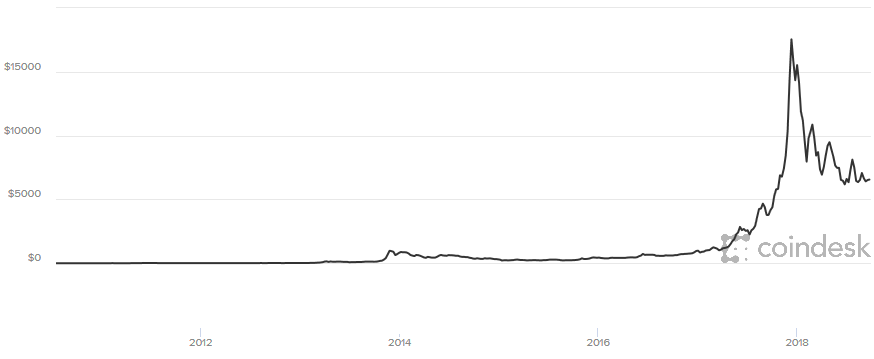
\includegraphics[scale=0.4]{\ImgPath/rys/bitcoin.png}
\end{center}
	\caption{Bitcoin price over years}
	\label{bitcoin}
\end{figure}

But financial prospects are not the aspects this thesis is concerned with. The most groundbreaking features the blockchain posses and which actually put it into the focus of modern computer science are anonymity and trustlessness.
\begin{itemize}
\item Anonymity: In the simplest implementations of blockchain such as bitcoin it is not possible to find any information of the user participating in the network. That is a simple consequence of relying purely on assymetric cryptography and no other requirement for allowing to interact with the network other than having a key pair. This simple feature has amazing implications in the real world. Every one in the world with internet connection can actually use blockchain. Coupled with the fact that cryptocurrencies can be used for value storage a way of escaping unstable national currencies has appeared for every human being. Recent example of that can be seen in Venezuela \cite{Venezuela}. There are also people who have found ways to use the anonymity in an illegal way. Silk road, the greatest illegal drug webshop accessible by TOR network has experienced a renaissance every since bitcoin payments have been implemented \cite{Silkroad}. 

\item Trustless: All of the currencies in our world are based on trust. The paper money has only a fraction of the value we assign to it. The numbers in our bank accounts have virtually no value. Currencies are simply are major agreement between all of the people on the world. In this world central parties are required such as banks which hold record of all transactions. We trust banks that when we ask them whether a person willing to buy from us has enough money, a true information will be sent to us. The double spending problem is solved this way. But blockchain has it's own mechanisms for this and thus allows us to omit the central party. We call the blockchain a trustless system because there is no trust required when interacting with other parties on the blockchain. Everything is taken care of by the computers, algorithms and protocols. The most grand example is Bitcoin itself which serves as a currency and a bank for all of the participants.
\end{itemize}

The element of blockchain technology that needs explanation is creation of a new block. As described earlier, in Bitcoin it is achieved by computing hashes of random numbers until a hash with certain amount of zeros at the beginning is reached. The whole process is commonly referred to as mining. This amount of zeros is called \textit{the difficulty}. The purpose of \textit{the difficulty} is to simply hold the rate of blocks being created constant. That is lower the difficulty when there are few miners and the transactions would be processed very slowly or increase the difficulty when everyone starts using supercomputers for mining. Currently, the rate is adjusted every 2016 mined blocks. More exact information about this topic can be found on bitcoin wiki \cite{Bitcoinwiki}. One important question that is left to be answered is: why do miners should bother with mining? Especially, why do people mine transactions which are not theirs? The answer is \textit{reward} and \textit{fees}. Currently, every mined block grants the miner who has done it some amount of bitcoin, that is a \textit{reward} for mining. Additionally, people simply willing to use Bitcoin for transaction purposes can attach fee to their transactions so that miners will be more likely to mine those transactions first and receive the fee. 

But looking for specific hashes is only one way of controlling block creation rate. PrimeCoin is especially worth noting as its method of mining is by finding prime numbers. Mining itself has also become a major part of computer hardware world due to computing power is has accumulated. Mining hashes is nowadays done only by GPUs due to parallelism benefits. There has been even created a special hardware called \textit{ASIC} which exist solely for the purpose of mining hashes.

After the subject of mining has been explained we encounter another problem. We know that after a block has been mined it has to be propagated throughout the network as to be actually accepted by the network.
What happens when in a large network two blocks are mined at the same time and both are able to propagate only through a part of the network before they collide? Then at least the majority of the miners ( that is 51\% of all computing power) has to decide which block to link to the blockchain and which to throw out. It is very important that a solid method of choosing the block by majority is used in a blockchain implementation because otherwise a malicious party could take over the network in some way or another by forcing his blocks with his transactions. It it also possible that the declined block will not be thrown away but will start living his own life in a sequence of events that are known as \textit{forks}. What follows is that one blockchain is split into two smaller ones which live from then on their own lives. Most of the time forks happen because a new version of the blockchain implementation is being deployed and not everyone wants this new version. This situation has occured with Bitcoin multiple times and the whole subject is worth thesis on its own.

Possible topics to elaborate:
\begin{itemize}
\item Comparing blockchain to sql and nosql? (trustlessness, no scalability)
\item What coins are there? (Bitcoin, Ethereum)
\item When to use blockchain? ( use cases )
\item How to take over the network?
\item Scalability solutions?
\end{itemize}

\section{Ethereum}

Ethereum is one of many implementations of blockchain technology. It differs from the many other ones in that it is as a next step in the evolution of blockchain. Learning from Bitcoin mistakes and trying to create a flawless general-purpose blockchain implementation, Vitalik Buterin together with other programmers have published a paper outlying desing for Ethereum \cite{Ethereum}.  The new cryptocurrency has been officially released in year 2015. 

Owing to a plethora of new features, among which smart contracts are most notable, Ethereum has managed to become one of the most widely known and used cryptocurrencies in the world. It was the first to acquire support of real-world corporations. There are also actual companies serving products based on Ethereum. Being one of the cryptocurrencies it has also became a big part of the financial cryptoworld and has gone trough phases of big volatility, which can be seen on the graph \ref{ethereum}

\begin{figure}[!htbp]
	\begin{center}
\centering
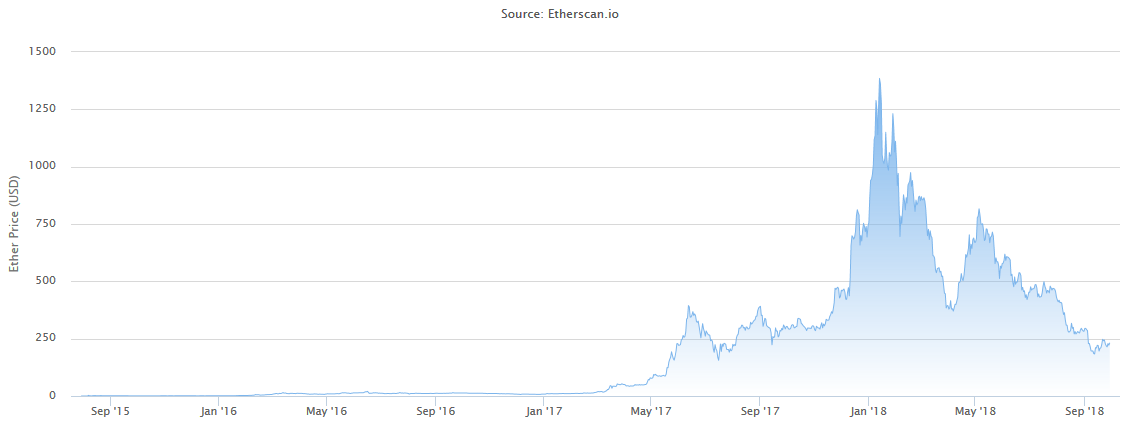
\includegraphics[scale=0.4]{\ImgPath/rys/ethereum.png}
\end{center}
	\caption{Ethereum price over years}
	\label{ethereum}
\end{figure}

The are a couple factors which make Ethereum unique and can be seen as an improvement over Bitcoin. 
\begin{itemize}
\item Faster and more scalable than Bitcoin: Every cryptocurrenct has scalability issues which stem from the fact that theoretically every network participant should posses the whole blockchain. But Ethereum team has gone one step ahead and started creating tweaks for this problem. While estimated peak performance of Bitcoin is that of seven transactions per second, Ethereum has managed to reach performance of twelve transactions per second. The most important fact tough is that constant research is being carried out which should find the solution for the scalability problem. So far the only discovered methods for solving this issue consist of sacrificing decentralization and thus security of the network.

\item Proof-of-Stake: As explained earlier, when two conflicting blocks meet on Bitcoin blockchain, the majority of miners have to decide which block to accept. This way of solving conflicts is called Proof-of-Work. The problem with this approach of using miners in general is that a lot of power is being used by the hardware around the world to power the different blockchains. The amount of power being used is apparently comparable to energy consumption of some smaller countries \cite{energy}.  Ethereum team is willing to change that by using Proof-of-Stake mechanism. This way the whole notion of mining is being eradicated. To create a new block a group of network participants is being asked to confirm transactions. The group has to be big enough so that the amount of coins they hold on specific blockchain sums up to 51\% of all the coins present on this blockchain. What follows is that only a fraction of the energy will be consumed and the network is still secure because a person willing to take over the network would have to buy 51\% of the coins on this blockchain. If we assume that market forces are working properly then the intruder probably will not have enough resources to carry out the attack. Nevertheless, it can be seen that we switch from one problem to another and users of Ethereum should be wary of that. 

\item Smart contracts: The single most important notion which differentiates Ethereum from all the other blockchain implementations is that of a smart contract. The general idea is that Ethereum blockchain has an Ethereum Virtual Machine(EVM) built into it. Which actually serves similar purpose as Java Virtual Machine for Java. If we put some lines of code of a language called Solidity into the transaction part of a block, the code will be executed after confirmation of this block. What smart contracts, EVM and solidity actually are will be explained in the next section. The most important fact is that thanks to this invention we are actually able to store not only static data in the blockchain but also code which will be executed. Thus, we acquire a fool-proof method of storing and carrying out procedures.
\end{itemize}

Immediate result of this invention are what's called Decentralized Applications(DAs) and Decentralized Autonomous Organizations(DAOs). If we call a typical blockchain a trustless database then we could call Ethereum blockchain coupled with solidity code a trustless application. Referring to a bank example mentioned earlier which can be replaced by blockchain for storing money but nothing more, we can see that now we are able to replace a banking entity also in such aspects as periodic payments or loans. Actually any operation which required intermediary can be now replaced by a piece of code which will be used by both side of the contract. The only requirement is that the deal has to use Ethereum and has to be carried out on the Etehereum platform. Fulfilment of those tasks can be achieved by construction of a Decentralized Application. 

If we go one step further we notice that is actually possible to create another cryptocurrency on top of Ethereum. Just as Ethereum is backed by a Proof-of-Work or a Proof-of-Stake we can create our own coins which will be backed by smart contracts, which in turn are backed by the Ethereum mechanisms. Those coins are most often called tokens. Finally, if a DA is created which facilitates it's own token we end up with a self living entity which trades its own money with it's own set of rules. That is what we call DAO.

As for the moment of writing this work there are almost two thousand DApps ( more popular naming of a DA ) serving purposes ranging from video games through social interactions up to financials \cite{dapps}.  Additionally, almost seven hundred tokens are being lively supported \cite{tokens}. 

Lastly, it is worthwhile to elaborate on the topic of cryptocurrency creation using smart contracts. The process goes by the name of Internal Coin Offering(ICO) which is taken straight from Initial Public Offering(IPO). IPO is simply what happens when company starts listing itself on the stock exchange. ICOs  pursue similar position as they mostly go hand in hand with a deployment of a fresh DAO. The coin offerings have become a vital part of the cryptocurrencies world as they have managed to earn millions of dollars and have become a new way for companies around the world to gain funding. Another sign of blockchain technology binding itself stronger to the world of real life usage.

\section{Smart contracts}

Smart contracts are files of code written in programming language called Solidity which are stored on blockchain and executed by Ethereum Virtual Machine(EVM). The specifications of the EVM will not be examined in this work as the material reaches outside of the aim of this thesis. Most of the information can found easily in the Ethereum yellow paper \cite{ethyellow}.  The notion of EVM will be touched upon in the last chapter where specific methods of code compilation will be described.

What needs explanation are the characteristics of Solidity language. It is an object-oriented, high-level language for implementing smart contracts. It's syntax has been influenced by C++, Python and JavaScript. Solidity is statically typed, supports inheritance, libraries and complex user-defined types among other features. Additionally, it is turing complete. It is very important to notice that blockchain serves overall a similar function to that of a database. But databases in general offer us SQL or SQL-like languages which are not turing complete without considerable extensions. Solidity in turn offers us a different perspective. We are able to experience a language which deals with directly with data storage but offers us the possibility to solve most computational problems at the same time. Of course SQL languages are declarative and operate on different types of data structures thus serve other purposes. But we can see that a new frontier has opened in the data storage world.

It is also important to understand the implications of programs running on blockchain. As every transaction done on blockchain has to be stored on blockchain it is also true that programs running on blockchain have to save their every change of the state on the blockchain. Thus the actions have to be confirmed by other users of the network and propagated. It is now possible to create program by a malicious user or by a bug which would spam the whole network and thus make it unusable. For example, an infinite loop in a smart contract would need constant confirmations and would not allow others to do anything with the network. To circumnavigate this problem a notion of \textit{gas} is introduced. Every smart contract put on the blockchain has to have some amount of Ether assigned to it. Every line of code run on this contract consumes gas. Different operations cost different amount of gas. For example, read operations cost no gas but sending ether from contract to somewhere else costs a lot of gas. The gas amounts can be found easily on the internet \cite{gas}.  The amount of gas respective operations consume is fixed. But the price of every gas unit denominated in Ether is subject to change. To run a line of code the contract has to pay product of amount of gas used and current gas price. The gas price is shaped by many factors but it is mostly set by miners. As a result the infinite loops would eventually run out of funds to consume and would stop. Moreover, usage of gas and not simply Ether lets those two values be decoupled. Thus a double increase of Ether value will not directly affect the gas price. Still, the gas price can change and thus we can see that big smart contracts are discouraged as they can become expensive to use. 

Just by this fact we can see that programming in Solidity is specific and requires careful considerations in many areas. Most notably those areas would be:
\begin{itemize}
\item Gas optimization: Besides cost of running code there also come costs of storing data. Because every variable or data structure used in a smart contract also comes with a cost. As a result we could notice a similarity to the old days of programming when computing power and more importantly storage space were scarce. A Solidity programmer also has to use a lot of tricks to keep his code small and fast. Unfortunately, the history of software development has shown that such practices often end up in a code that looks badly and is unmaintainable. Remedy for possible future catastrophes could be usage of open-source libraries which hold optimal fault-proof solutions, future developments in language which would abstract the gas optimization away and extensive testing.
\item Security: Ethereum is all about money and the end purpose of Solidity is automation of money handling processes. An immediate consequence of those facts is that Ethereum world is a breeding ground of malicious users which will use every possible loop-hole in the system to steal the biggest possible amount of funds possible and then perish behind the veil of anonymity. The problem with stealing on blockchain is that once it is done it is done. If we are not able to connect the public address of the hacker with his real world identity then there is nothing we can really do. Moreover, the gas optimization practices stimulate creation of unsecure code. Fortunately, the issue has been noticed by the community and there are plenty of materials allowing for education in those matters. The documentation of Solidity being a good starting point \cite{secure}. 
\item Bugs: Solidity is one of the most costly language in the world when it comes to bugs. One bad mathematical operation could create a completely wrong address of transaction receiver and thus result in a transfer of millions of dollars to a dead account. It has happened before and is still happening. Testing is one of the most vital aspects of Solidity programming and an aim of 200\% test coverage should not be treated as a joke. It is also a good practice to use private test blockchain networks where funds can be created out of thin air. Those networks can be used for integration testing and such. Ethereum itself offers three world-wide networks besides the main one which only purpose is letting user test their contracts and letting Ethereum developers test new solutions. These networks are named Ropsten, RinkeBy and Kovan. 
\end{itemize}

It is obligatory for the language to allow for a communication with an outside world. That is to allow for external parties to read the blockchain data and interact with the blockchain state. The task is achieved by a Remote Procedure Call(RPC) communication as well as by Inter Process Communication(IPC). In this work the RPC variant is being used and explained due to it's versatility. The messages used are simply JSONs. The whole API reference can be found on ethereum wiki \cite{RPC}.  Our client has to connect to an Ethereum node which serves and appropriate end-point through HTTP. As the API is quite simple a ready implementation of the communicator can be found in most of the widely used programming languages. The general standard of RPC messaging used by Ethereum goes by the name web3. As this project used Java, the library web3j was used. Still, web3.js for JavaScript or web3.py for Python could have been used as well.

%-----------------
% Current state of the technology
%-----------------
\chapter{Current state of the technology}

In this project blockchain will be used to enable decentralized and trustless loan servicing. The idea of transferring this major business into the crypto world has quickly become one of the first use cases of the technology. As such, it is possible to observe a multitude of solutions present on the market. Each coming with it's own innovative mechanisms, it's own strengths and it's own weaknesses. Generally, there are two main points differentiating approaches to this problem. 

Firstly, it is noticeable that most of the loan service providers specialise in one certain branch of the loan business and offer services in only this branch. For example, there are companies offering just normal loans to people in need of money whereas the cash to lend is provided by people willing to invest their money. Some other companies organizations focus only on letting you leverage your trading by usage of loans. Finally, there are some cases of business offering possibility to automate real life loan processes using blockchain.     

Secondly, everyone has it's own approach to dealing with the problem of lack of loan repayments. When a person lends money to someone he immediately wages a risk that the borrower could go default and could stop repaying his loan. Leaving the lender with nothing. Situation especially dire in the world of blockchain where it is not so easy to reclaim your money on your own. Fortunately, some remedies to this problem have been found and are widely used. The example being, backing your loans with collaterals or sharing your personal data for the sake of possible legal procedures.

In this chapter some of the most prominent products or systems will be presented and grouped according to the two points mentioned above.

\section{Normal loans}
The first group concerns typical loans. The kind that first comes to our mind when somebody hears the world \textit{loan}. The only difference here is that the entity providing loans is not some company but other people.  In this business model the companies provide the technology for matching the borrowers and lenders or help lenders have their money back. For this they receive minor fees. All of the processes related to granting loans or setting interest rates are automated and controlled by the market forces.
One could ask, what is the difference between those firms and the ones not using blockchain for this type of loan providing? The answer is that if the cryptocompany resorts to a minimal usage of cryptocurrencies it will still automate the loan contract itself. Therefore, no legal documents are really required as all of the essential financial procedures are saved on the blockchain. Traditional company will always have to create some legally binding document which in the essence will be based on trust between borrowers and lenders.

Beginning, a company named \textit{ETHLend} \cite{ethlend} is examined. Created at the brink of the year 2017 ETHLend has, so far, successfully implemented the idea described above. The whole system is based on Ethereum and allows for deals using Ethereum or tokens based on it. Users create their anonymous accounts to which credit history is slowly accumulated with progression of time and repaid loans. The loans require a collateral which will amount to some part of the loan. The collateral is most often some other cryptocurrency. We can see that in the essence, the company simply allows us to leverage our holding by exchanging the currency at the same time. Additionally, an ICO of a coin named \textit{LEND} has been carried out at the inauguration of the company. The funds gained during the ICO have been used to cover expenses of the company and invest for future development. Moreover, the LEND token can be also used for lending and allows for some extra functionalities of the system. ETHLend is an interesting example of blockchain company successfully using the technology to fill business needs and properly finance itself.

\url{}
\url{https://btcpop.co/home.php}
\url{https://www.bitbond.com/}
\url{https://crediblefriends.com/}

\section{Cash for coins}
\url{https://www.kambo.io/}
\url{https://www.unchained-capital.com/}
\url{https://saltlending.com/}

\section{Leverage}
\url{https://makerdao.com/}

\section{Loan automation}
\url{https://www.othera.io/}

%-----------------
% Software design
%-----------------
\chapter{Software design}

\section{Loans}
One loan offer on an exchange will consist of following parameters:
\begin{itemize}
\item \textbf{Basis}: Size of the loan denominated in Ethereum.
\item \textbf{Duration}: The time after which the whole loan should be paid back together with interest. Depicted per predefined amount of days.
\item \textbf{Interest}: Percentage of the loan basis which has to be additionally paid by loan taker. Calculated per predefined amount of days.
\item \textbf{Collateral}: Information whether the loan is backed by a third party and has a low probability of going default. For example loan taker with no evidence to back his repayment probability will have only access to loans with collateral parameter being equal to None. At the same time loan taker with his loan being backed by a special bank agreement whereas there is a deposit with amount equal to the loan basis and interest incurred which is connected to a smart contract will have access to loans with collateral being equal to Yes.
\end{itemize}

The process of buying and selling loans will have the same characteristics as the one seen on the stock exchange. 

That is loan ask whose size exceeds size of one respective loan bid will automatically cover the second identical loan bid. For example loan taker A asks for a loan of 1 ETH. There are two identical offers by loan provider B and C both equal to 0.5 ETH. The matching will automatically buy for A both loans from B and C.

Moreover, if loan taker asks for a loan of interest higher than the lowest present on the market he will be sold the loan with the lowest interest. For example loan taker asks for a loan of interest 2\%. There are loans on the market being bid with both interest of 2\% and 1\%. The loan of 1\% will be sold to the loan taker.

In terms of repayments the loan will function as an amortized loans. That is, the repayments will be constant with principal amount being paid back increasing and the interest amount decreasing. The formula for computing the installments looks as follows:
\[C = \frac{rP}{1 - \frac{1}{(1+r)^n}}\]
Where C is monthly installment, r is interest rate per month, P is principal amount/basis and n is a duration of a loan in periods equal to predefined amount of days.

\section{Types of users}

The project provides for three types of possible actors. They are as follows:
\begin{itemize}
\item \textbf{Loan providers}: Any user with spare Ethereum and access to the application. Such person bids his loan offer and once the loan is sold automatic processes backed by smart contracts care for repayments.
\item \textbf{Loan takers}: User who has fulfilled required information inquires and can be assured of that at least one of the methods of repayment can be exercised on him. The methods are:
\begin{enumerate}
\item Regular individual refilling of his repayment account.
\item Usage of a collateral deposit from a third party.
\item Following legal procedures by bailiff of a country where the loan taker is located.
\end{enumerate}
\item \textbf{Authorities}: Third parties which for example serve the role of a collateral deposit or bailiff chasing the loan taker. This user has the possibility to refill the account of the loan takers repayment account.
\end{itemize}


\section{Processes}

\section{Requirements}
The complete system should provide following functions:
\begin{enumerate}
\item Loan providers and loan takers should be able to:
\begin{itemize}
\item check and transfer funds to and from their accounts using external wallet based on Ethereum network.
\item specify the following parameters in their loan bids and asks: Basis, Duration, Interest, whether it has collateral.
\item check their open bids and asks as well as the whole public exchange.
\item cancel all of their open bids and asks.
\end{itemize}
\item Loan takers should be able to:
\begin{itemize}
\item specify legal informations which could be used by bailiff if repayment did not happen. At the same time the information should remain confidential so long there is no need to use them.
\item bind his account with an account of a third party. The additional account will always hold a sum required to repay the whole loan when needed.
\item repay the loan earlier.
\end{itemize}
\item Every user should be able to:
\begin{itemize}
\item access the application having only internet connection.
\item maintain his anonymity while using the system.
\end{itemize}
\end{enumerate}



\section{Architecture}

\section{Visuals}
%-----------------
% Software implementation
%-----------------
\chapter{Software implementation}

\section{Ethereum network}
What is Geth?
What is ganache-cli?


\section{Solidity}

How to compile?
What is truffle?
Math without decimals and negative numbers?
How to compute exponential?

\subsection*{Safety}
How to transfer funds? 
What is condition-computation-action?
What are public operators?

\subsection*{Tests}
Js tests?
Solidity tests?


\section{Java}

How to compile?


\section{Completion verification}
How to compile?

\begin{thebibliography}{99}
\addcontentsline{toc}{chapter}{Bibliography}
\bibitem{Bitcoin}{Satoshi Nakamoto , Access date: 02.10.2018 , ,,Bitcoin: A Peer-to-Peer Electronic Cash System'', \url{https://bitcoin.org/bitcoin.pdf}}
\bibitem{Venezuela}{Simon Chandler, Access date: 02.10.2018, ,,How Venezuela Came to Be One of the Biggest Markets for Crypto in the World'', \url{https://goo.gl/s1t7nm}}
\bibitem{Silkroad}{Silk Road Drugs, Access date: 02.10.2018, ,,The Effect Of Silk Road On Bitcoin And Tor'', \url{https://silkroaddrugs.org/the-effect-of-silk-road-on-bitcoin-and-tor/}}
\bibitem{Bitcoinwiki}{Access date: 02.10.2018, \url{https://en.bitcoin.it/wiki/Difficulty}}
\bibitem{Ethereum}{Access date: 02.10.2018, \url{https://github.com/ethereum/wiki/wiki/White-Paper}}
\bibitem{energy}{Access date: 02.10.2018, \url{https://digiconomist.net/bitcoin-energy-consumption}}
\bibitem{dapps}{Access date: 02.10.2018, \url{https://www.stateofthedapps.com/}}
\bibitem{tokens}{Access date: 02.10.2018, \url{https://etherscan.io/tokens}}
\bibitem{ethyellow}{Gavin Wood, Access date: 02.10.2018, \url{https://gavwood.com/paper.pdf}}
\bibitem{gas}{Access date: 02.10.2018, \url{https://github.com/djrtwo/evm-opcode-gas-costs}}
\bibitem{secure}{Access date: 02.10.2018, \url{https://solidity.readthedocs.io/en/v0.4.24/security-considerations.html}}
\bibitem{RPC}{Access date: 02.10.2018, \url{https://github.com/ethereum/wiki/wiki/JSON-RPC}}
\bibitem{ethlend}{Access date: 03.10.2018, \url{https://ethlend.io/#/main}}

\end{thebibliography}

\zakonczenie  % wklejenie recenzji i opinii

\end{document}
%+++ END +++
